
\section*{Problema P9.3}

\renewcommand*\thesection{9.3}
\numberwithin{equation}{section}

\begin{center}
    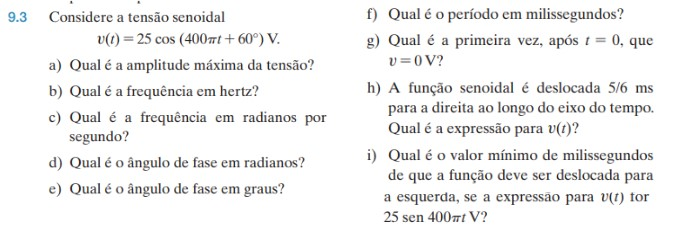
\includegraphics[scale=1.0]{P9.3.jpg}
\end{center}

\subsection*{(a)}

Sabemos que uma tensão senoidal $v(t)$ é expressa na forma


\begin{equation}\label{eq:9.3.1}
    v(t) = A\cos\left(\omega t + \phi\right)
\end{equation}

onde

\begin{itemize}
    \item $A$: amplitude máxima da tensão (V);
    \item $\omega$: frequência angular da tensão (rad/s);
    \item $\phi$: defasagem em relação à origem (rad ou °).
\end{itemize}

Portanto, conforme o enunciado, temos

\[ \boxed{A = 25 \un{V}}  \]

\subsection*{(b)}

A frequência angular $\omega$ é dada por

\[ \omega = 2\pi f \quad \Rightarrow \quad f = \frac{\omega}{2\pi} \]

Substituindo, temos

\[ \boxed{f = 200 \un{Hz}}  \]

\subsection*{(c)}

Conforme o enunciado, temos

\[ \boxed{\omega = 400\pi \un{rad/s} = 1256.64 \un{rad/s}}  \]

\subsection*{(d)}

Conforme o enunciado, temos $\phi = 60^{\circ}$. Convertendo para radianos, temos

\[ \boxed{\phi = \frac{\pi}{3} \un{rad} = 1.047 \un{rad}}  \]

\subsection*{(e)}

Conforme o enunciado,

\[ \boxed{\phi = 60^{\circ}}  \]

\subsection*{(f)}

A frequência angular $\omega$ é dada por

\[ \omega = 2\pi f \quad \Rightarrow \quad \omega = \frac{2\pi}{T} \quad \Rightarrow \quad T = \frac{2\pi}{\omega}\]

Substituindo,

\[ \boxed{T = 5 \un{ms}}  \]

\subsection*{(g)}

Isolando $t$ em \eqref{eq:9.3.1}, temos

\[ \omega t + \phi = \cos^{-1}\left(\frac{v(t)}{A}\right) \]

\begin{equation}\label{eq:9.3.2}
    t = \frac{1}{\omega} \left[\cos^{-1}\left(\frac{v(t)}{A}\right) - \phi \right]
\end{equation}

Para identificar os instantes $t$ para os quais $v(t)=0$, substituímos $v(t)=0$ em \eqref{eq:9.3.2}, obtendo

\[  t = \frac{1}{\omega} \left[\cos^{-1}\left(0\right) - \phi \right] \]

O primeiro ângulo $\theta$ para o qual $cos(\theta) = 0$ é $\frac{\pi}{2}$, portanto  

\[  t = \frac{1}{\omega} \left[\frac{\pi}{2} - \phi \right] \]

Substituindo os valores do enunciado, temos

\[ \boxed{t = 416.67 \;\mu\textrm{s}}  \]

\subsection*{(h)}

Do item (f), sabemos que $T=5ms$. Além disso, sabemos que $1T=360^{\circ}$ para a função cosseno. 
Portanto, usando proporcionalidade, temos

\[ \frac{T}{\Delta t} = \frac{360^{\circ}}{\Delta \phi}  \]

Substituindo,

\[ \frac{5 \un{ms}}{\frac{5}{6} \un{ms}} = \frac{360^{\circ}}{\Delta \phi}  \]

\[ \Delta \phi = 60^{\circ}  \]

Portanto, um deslocamento de $\frac{5}{6} \un{ms}$ equivale a um deslocamento angular de $\Delta \phi = 60^{\circ}$.
Note que deslocamentos à direita de uma função trigonométrica correspondem a deslocamentos com sinal negativo. Assim, 

\[ \Delta \phi = -60^{\circ}  \]

Aplicando isso à função original, temos a nova expressão de $v(t)$ dada por

\[ v(t) = A\cos\left(\omega t + \phi + \Delta \phi\right) \]

\[ v(t) = 25\cos\left(400\pi t + 60^{\circ} - 60^{\circ}\right) \]

\[ \boxed{v(t) = 25\cos\left(400\pi t\right)  \un{V}}  \]

\subsection*{(i)}

Sabemos que

\[ \cos(\theta) = \sin(\theta + 90^{\circ}) \]

Portanto, podemos reescrever a função de $v(t)$ como

\[ v(t) = A\sin\left(\omega t + \phi + 90^{\circ}\right)  \]

Seja $\Delta t$ o deslocamento ao longo do eixo $x$ que provoca uma diferença de fase $\Delta\theta$, de tal modo que

\[ A\sin\left(\omega t + \phi + \Delta\theta + 90^{\circ}\right) =  A\sin\left(\omega t\right)  \]

Para isso, precisamos de

\[ \phi + \Delta\theta + 90^{\circ} = 0 \]

Portanto,

\[ \Delta\theta = - \phi - 90^{\circ} \]

Uma vez conhecido $\Delta\theta$, identificamos o deslocamento temporal $\Delta t$ através da proporcionalidade

\[ \frac{T}{\Delta t} = \frac{360^{\circ}}{- \phi - 90^{\circ}}  \]

Isolando $\Delta t$, temos

\[ \Delta t = (- \phi - 90^{\circ}) \frac{T}{360^{\circ}} \]

Substituindo,

\[ \boxed{\Delta t = - 2.08\un{ms}}  \]

